\title{Homework 5 Solutions for Computer Logic and Circuit Design: PHYS306/COSC330}
\author{Dr. Jordan Hanson - Whittier College Dept. of Physics and Astronomy}
\date{\today}
\documentclass[10pt]{article}
\usepackage[a4paper, total={18cm, 27cm}]{geometry}
\usepackage{graphicx}
\begin{document}
\maketitle

\section{6-2: Parallel Binary Adders}

\begin{enumerate}
\item Exercise 4: $C_{out} = 1$, $\Sigma_3 = 1$, $\Sigma_2 = 0$, $\Sigma_1 = 0$.
\item Exercise 5: $\Sigma_6 = 1$, $\Sigma_5 = 1$, $\Sigma_4 = 1$, $\Sigma_3 = 0$, $\Sigma_2 = 0$, $\Sigma_1 = 0$.
\item Exercise 8: See Fig. \ref{fig:wave1}.
\begin{figure}[ht]
\centering
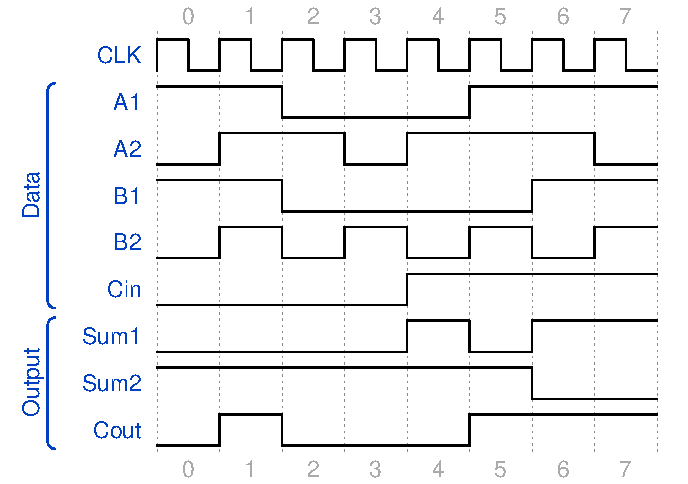
\includegraphics[width=0.35\textwidth]{code/hmk5_6-2-8.pdf}
\caption{\label{fig:wave1} Solution to exercise 8.}
\end{figure}
\end{enumerate}

\section{6-3: Ripple-Carry Adders}

\begin{enumerate}
\item Exercise 11: The first stage is limited by 40 ns delay between inputs and $C_{out}$.  Then, each in-between stage is limited by the 25 ns delay between $C_{in}$ and $C_{out}$. The exception is the last one, which is limited only by $C_{in}$ to $\Sigma$.  Thus, $40 + 6*25 + 35$ ns = 225 ns.
\end{enumerate}

\section{6-4: Comparators}

\begin{enumerate}
\item Exercise 13: See Fig. \ref{fig:wave2}.
\begin{figure}[hb]
\centering
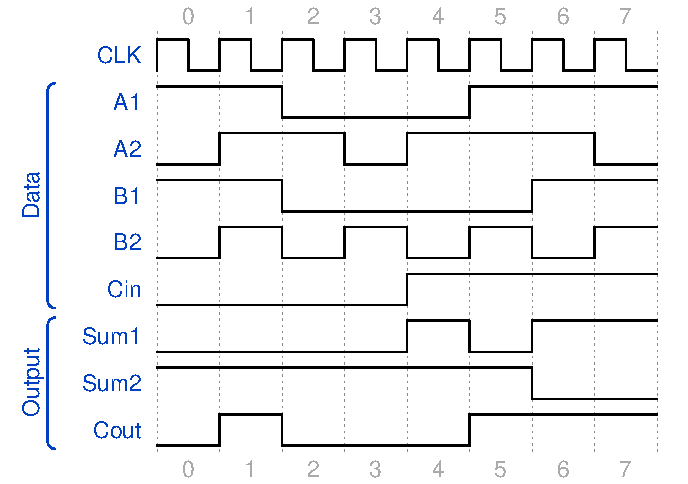
\includegraphics[width=0.25\textwidth]{code/hmk5_6-2-8.pdf}
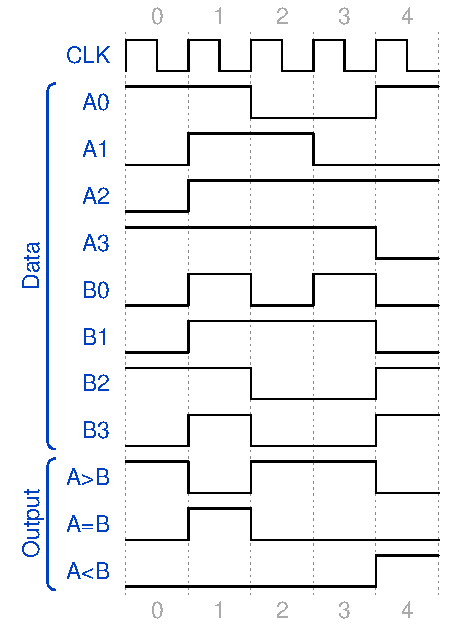
\includegraphics[width=0.25\textwidth]{code/hmk5_6-4-14.pdf}
\caption{\label{fig:wave2} (Left) Solution to E xercise 13.  (Right) Solution to Exercise 14.}
\end{figure}
\item Exercise 14: See Fig. \ref{fig:wave2}.
\end{enumerate}

\section{6-5: Decoders}

\begin{enumerate}
\item Exercise 16: a) 1110 b) 1100 c) 1111 d) 1000
\item Exercise 17: See Fig. \ref{fig:wave3}.
\begin{figure}
\centering
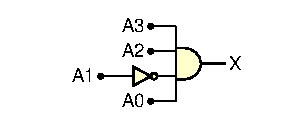
\includegraphics[width=0.25\textwidth]{code/hmk5_6-5-17a.pdf}
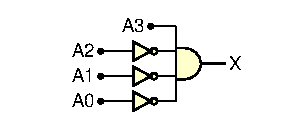
\includegraphics[width=0.25\textwidth]{code/hmk5_6-5-17b.pdf}
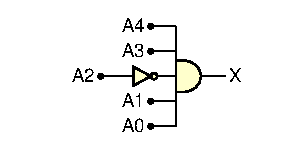
\includegraphics[width=0.25\textwidth]{code/hmk5_6-5-17c.pdf}
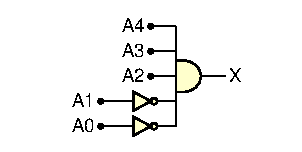
\includegraphics[width=0.25\textwidth]{code/hmk5_6-5-17d.pdf}
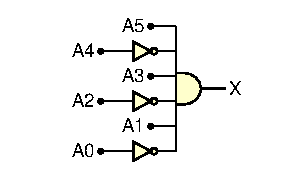
\includegraphics[width=0.25\textwidth]{code/hmk5_6-5-17e.pdf}
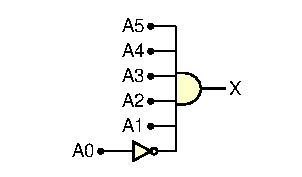
\includegraphics[width=0.25\textwidth]{code/hmk5_6-5-17f.pdf}
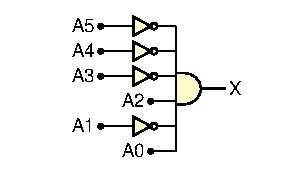
\includegraphics[width=0.25\textwidth]{code/hmk5_6-5-17g.pdf}
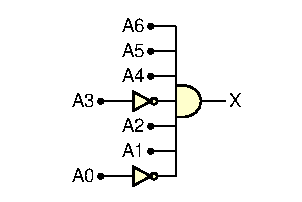
\includegraphics[width=0.25\textwidth]{code/hmk5_6-5-17h.pdf}
\caption{\label{fig:wave3} Solution to Exercise 17.}
\end{figure}
\item Exercise 19: Using the Karnaugh map, and the starting expression $X = A_3 \bar{A_2} A_1 \bar{A_0} + A_3 A_2 \bar{A_1} \bar{A_0} + \bar{A_3} \bar{A_2} \bar{A_1} A_0 + A_3 \bar{A_2} A_1 A_0$, we can show that the minimum logic is $X = \bar{A_3} \bar{A_2} \bar{A_1} A_0 + A_3 A_2 \bar{A_1} \bar{A_0} + A_3 \bar{A_2} A_1$.  See Fig. \ref{fig:wave4}.
\begin{figure}
\centering
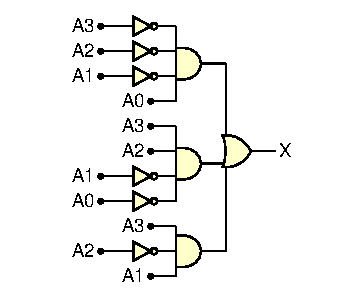
\includegraphics[width=0.25\textwidth]{code/hmk5_6-5-19.pdf}
\caption{\label{fig:wave4} Solution to Exercise 19.}
\end{figure}
\end{enumerate}

\section{6-6: Encoders}

\begin{enumerate}
\item No, because the output would be $A_3 A_2 A_1 A_0 = 1011$, or 11, which is not a valid BCD code.
\end{enumerate}

\end{document}
